
\documentclass[10pt]{article} % For LaTeX2e
\usepackage[accepted]{tmlr}
% If accepted, instead use the following line for the camera-ready submission:
%\usepackage[accepted]{tmlr}
% To de-anonymize and remove mentions to TMLR (for example for posting to preprint servers), instead use the following:
%\usepackage[preprint]{tmlr}

% Optional math commands from https://github.com/goodfeli/dlbook_notation.
%%%%% NEW MATH DEFINITIONS %%%%%

\usepackage{amsmath,amsfonts,bm}

% Mark sections of captions for referring to divisions of figures
\newcommand{\figleft}{{\em (Left)}}
\newcommand{\figcenter}{{\em (Center)}}
\newcommand{\figright}{{\em (Right)}}
\newcommand{\figtop}{{\em (Top)}}
\newcommand{\figbottom}{{\em (Bottom)}}
\newcommand{\captiona}{{\em (a)}}
\newcommand{\captionb}{{\em (b)}}
\newcommand{\captionc}{{\em (c)}}
\newcommand{\captiond}{{\em (d)}}

% Highlight a newly defined term
\newcommand{\newterm}[1]{{\bf #1}}


% Figure reference, lower-case.
\def\figref#1{figure~\ref{#1}}
% Figure reference, capital. For start of sentence
\def\Figref#1{Figure~\ref{#1}}
\def\twofigref#1#2{figures \ref{#1} and \ref{#2}}
\def\quadfigref#1#2#3#4{figures \ref{#1}, \ref{#2}, \ref{#3} and \ref{#4}}
% Section reference, lower-case.
\def\secref#1{section~\ref{#1}}
% Section reference, capital.
\def\Secref#1{Section~\ref{#1}}
% Reference to two sections.
\def\twosecrefs#1#2{sections \ref{#1} and \ref{#2}}
% Reference to three sections.
\def\secrefs#1#2#3{sections \ref{#1}, \ref{#2} and \ref{#3}}
% Reference to an equation, lower-case.
\def\eqref#1{equation~\ref{#1}}
% Reference to an equation, upper case
\def\Eqref#1{Equation~\ref{#1}}
% A raw reference to an equation---avoid using if possible
\def\plaineqref#1{\ref{#1}}
% Reference to a chapter, lower-case.
\def\chapref#1{chapter~\ref{#1}}
% Reference to an equation, upper case.
\def\Chapref#1{Chapter~\ref{#1}}
% Reference to a range of chapters
\def\rangechapref#1#2{chapters\ref{#1}--\ref{#2}}
% Reference to an algorithm, lower-case.
\def\algref#1{algorithm~\ref{#1}}
% Reference to an algorithm, upper case.
\def\Algref#1{Algorithm~\ref{#1}}
\def\twoalgref#1#2{algorithms \ref{#1} and \ref{#2}}
\def\Twoalgref#1#2{Algorithms \ref{#1} and \ref{#2}}
% Reference to a part, lower case
\def\partref#1{part~\ref{#1}}
% Reference to a part, upper case
\def\Partref#1{Part~\ref{#1}}
\def\twopartref#1#2{parts \ref{#1} and \ref{#2}}

\def\ceil#1{\lceil #1 \rceil}
\def\floor#1{\lfloor #1 \rfloor}
\def\1{\bm{1}}
\newcommand{\train}{\mathcal{D}}
\newcommand{\valid}{\mathcal{D_{\mathrm{valid}}}}
\newcommand{\test}{\mathcal{D_{\mathrm{test}}}}

\def\eps{{\epsilon}}


% Random variables
\def\reta{{\textnormal{$\eta$}}}
\def\ra{{\textnormal{a}}}
\def\rb{{\textnormal{b}}}
\def\rc{{\textnormal{c}}}
\def\rd{{\textnormal{d}}}
\def\re{{\textnormal{e}}}
\def\rf{{\textnormal{f}}}
\def\rg{{\textnormal{g}}}
\def\rh{{\textnormal{h}}}
\def\ri{{\textnormal{i}}}
\def\rj{{\textnormal{j}}}
\def\rk{{\textnormal{k}}}
\def\rl{{\textnormal{l}}}
% rm is already a command, just don't name any random variables m
\def\rn{{\textnormal{n}}}
\def\ro{{\textnormal{o}}}
\def\rp{{\textnormal{p}}}
\def\rq{{\textnormal{q}}}
\def\rr{{\textnormal{r}}}
\def\rs{{\textnormal{s}}}
\def\rt{{\textnormal{t}}}
\def\ru{{\textnormal{u}}}
\def\rv{{\textnormal{v}}}
\def\rw{{\textnormal{w}}}
\def\rx{{\textnormal{x}}}
\def\ry{{\textnormal{y}}}
\def\rz{{\textnormal{z}}}

% Random vectors
\def\rvepsilon{{\mathbf{\epsilon}}}
\def\rvtheta{{\mathbf{\theta}}}
\def\rva{{\mathbf{a}}}
\def\rvb{{\mathbf{b}}}
\def\rvc{{\mathbf{c}}}
\def\rvd{{\mathbf{d}}}
\def\rve{{\mathbf{e}}}
\def\rvf{{\mathbf{f}}}
\def\rvg{{\mathbf{g}}}
\def\rvh{{\mathbf{h}}}
\def\rvu{{\mathbf{i}}}
\def\rvj{{\mathbf{j}}}
\def\rvk{{\mathbf{k}}}
\def\rvl{{\mathbf{l}}}
\def\rvm{{\mathbf{m}}}
\def\rvn{{\mathbf{n}}}
\def\rvo{{\mathbf{o}}}
\def\rvp{{\mathbf{p}}}
\def\rvq{{\mathbf{q}}}
\def\rvr{{\mathbf{r}}}
\def\rvs{{\mathbf{s}}}
\def\rvt{{\mathbf{t}}}
\def\rvu{{\mathbf{u}}}
\def\rvv{{\mathbf{v}}}
\def\rvw{{\mathbf{w}}}
\def\rvx{{\mathbf{x}}}
\def\rvy{{\mathbf{y}}}
\def\rvz{{\mathbf{z}}}

% Elements of random vectors
\def\erva{{\textnormal{a}}}
\def\ervb{{\textnormal{b}}}
\def\ervc{{\textnormal{c}}}
\def\ervd{{\textnormal{d}}}
\def\erve{{\textnormal{e}}}
\def\ervf{{\textnormal{f}}}
\def\ervg{{\textnormal{g}}}
\def\ervh{{\textnormal{h}}}
\def\ervi{{\textnormal{i}}}
\def\ervj{{\textnormal{j}}}
\def\ervk{{\textnormal{k}}}
\def\ervl{{\textnormal{l}}}
\def\ervm{{\textnormal{m}}}
\def\ervn{{\textnormal{n}}}
\def\ervo{{\textnormal{o}}}
\def\ervp{{\textnormal{p}}}
\def\ervq{{\textnormal{q}}}
\def\ervr{{\textnormal{r}}}
\def\ervs{{\textnormal{s}}}
\def\ervt{{\textnormal{t}}}
\def\ervu{{\textnormal{u}}}
\def\ervv{{\textnormal{v}}}
\def\ervw{{\textnormal{w}}}
\def\ervx{{\textnormal{x}}}
\def\ervy{{\textnormal{y}}}
\def\ervz{{\textnormal{z}}}

% Random matrices
\def\rmA{{\mathbf{A}}}
\def\rmB{{\mathbf{B}}}
\def\rmC{{\mathbf{C}}}
\def\rmD{{\mathbf{D}}}
\def\rmE{{\mathbf{E}}}
\def\rmF{{\mathbf{F}}}
\def\rmG{{\mathbf{G}}}
\def\rmH{{\mathbf{H}}}
\def\rmI{{\mathbf{I}}}
\def\rmJ{{\mathbf{J}}}
\def\rmK{{\mathbf{K}}}
\def\rmL{{\mathbf{L}}}
\def\rmM{{\mathbf{M}}}
\def\rmN{{\mathbf{N}}}
\def\rmO{{\mathbf{O}}}
\def\rmP{{\mathbf{P}}}
\def\rmQ{{\mathbf{Q}}}
\def\rmR{{\mathbf{R}}}
\def\rmS{{\mathbf{S}}}
\def\rmT{{\mathbf{T}}}
\def\rmU{{\mathbf{U}}}
\def\rmV{{\mathbf{V}}}
\def\rmW{{\mathbf{W}}}
\def\rmX{{\mathbf{X}}}
\def\rmY{{\mathbf{Y}}}
\def\rmZ{{\mathbf{Z}}}

% Elements of random matrices
\def\ermA{{\textnormal{A}}}
\def\ermB{{\textnormal{B}}}
\def\ermC{{\textnormal{C}}}
\def\ermD{{\textnormal{D}}}
\def\ermE{{\textnormal{E}}}
\def\ermF{{\textnormal{F}}}
\def\ermG{{\textnormal{G}}}
\def\ermH{{\textnormal{H}}}
\def\ermI{{\textnormal{I}}}
\def\ermJ{{\textnormal{J}}}
\def\ermK{{\textnormal{K}}}
\def\ermL{{\textnormal{L}}}
\def\ermM{{\textnormal{M}}}
\def\ermN{{\textnormal{N}}}
\def\ermO{{\textnormal{O}}}
\def\ermP{{\textnormal{P}}}
\def\ermQ{{\textnormal{Q}}}
\def\ermR{{\textnormal{R}}}
\def\ermS{{\textnormal{S}}}
\def\ermT{{\textnormal{T}}}
\def\ermU{{\textnormal{U}}}
\def\ermV{{\textnormal{V}}}
\def\ermW{{\textnormal{W}}}
\def\ermX{{\textnormal{X}}}
\def\ermY{{\textnormal{Y}}}
\def\ermZ{{\textnormal{Z}}}

% Vectors
\def\vzero{{\bm{0}}}
\def\vone{{\bm{1}}}
\def\vmu{{\bm{\mu}}}
\def\vtheta{{\bm{\theta}}}
\def\va{{\bm{a}}}
\def\vb{{\bm{b}}}
\def\vc{{\bm{c}}}
\def\vd{{\bm{d}}}
\def\ve{{\bm{e}}}
\def\vf{{\bm{f}}}
\def\vg{{\bm{g}}}
\def\vh{{\bm{h}}}
\def\vi{{\bm{i}}}
\def\vj{{\bm{j}}}
\def\vk{{\bm{k}}}
\def\vl{{\bm{l}}}
\def\vm{{\bm{m}}}
\def\vn{{\bm{n}}}
\def\vo{{\bm{o}}}
\def\vp{{\bm{p}}}
\def\vq{{\bm{q}}}
\def\vr{{\bm{r}}}
\def\vs{{\bm{s}}}
\def\vt{{\bm{t}}}
\def\vu{{\bm{u}}}
\def\vv{{\bm{v}}}
\def\vw{{\bm{w}}}
\def\vx{{\bm{x}}}
\def\vy{{\bm{y}}}
\def\vz{{\bm{z}}}

% Elements of vectors
\def\evalpha{{\alpha}}
\def\evbeta{{\beta}}
\def\evepsilon{{\epsilon}}
\def\evlambda{{\lambda}}
\def\evomega{{\omega}}
\def\evmu{{\mu}}
\def\evpsi{{\psi}}
\def\evsigma{{\sigma}}
\def\evtheta{{\theta}}
\def\eva{{a}}
\def\evb{{b}}
\def\evc{{c}}
\def\evd{{d}}
\def\eve{{e}}
\def\evf{{f}}
\def\evg{{g}}
\def\evh{{h}}
\def\evi{{i}}
\def\evj{{j}}
\def\evk{{k}}
\def\evl{{l}}
\def\evm{{m}}
\def\evn{{n}}
\def\evo{{o}}
\def\evp{{p}}
\def\evq{{q}}
\def\evr{{r}}
\def\evs{{s}}
\def\evt{{t}}
\def\evu{{u}}
\def\evv{{v}}
\def\evw{{w}}
\def\evx{{x}}
\def\evy{{y}}
\def\evz{{z}}

% Matrix
\def\mA{{\bm{A}}}
\def\mB{{\bm{B}}}
\def\mC{{\bm{C}}}
\def\mD{{\bm{D}}}
\def\mE{{\bm{E}}}
\def\mF{{\bm{F}}}
\def\mG{{\bm{G}}}
\def\mH{{\bm{H}}}
\def\mI{{\bm{I}}}
\def\mJ{{\bm{J}}}
\def\mK{{\bm{K}}}
\def\mL{{\bm{L}}}
\def\mM{{\bm{M}}}
\def\mN{{\bm{N}}}
\def\mO{{\bm{O}}}
\def\mP{{\bm{P}}}
\def\mQ{{\bm{Q}}}
\def\mR{{\bm{R}}}
\def\mS{{\bm{S}}}
\def\mT{{\bm{T}}}
\def\mU{{\bm{U}}}
\def\mV{{\bm{V}}}
\def\mW{{\bm{W}}}
\def\mX{{\bm{X}}}
\def\mY{{\bm{Y}}}
\def\mZ{{\bm{Z}}}
\def\mBeta{{\bm{\beta}}}
\def\mPhi{{\bm{\Phi}}}
\def\mLambda{{\bm{\Lambda}}}
\def\mSigma{{\bm{\Sigma}}}

% Tensor
\DeclareMathAlphabet{\mathsfit}{\encodingdefault}{\sfdefault}{m}{sl}
\SetMathAlphabet{\mathsfit}{bold}{\encodingdefault}{\sfdefault}{bx}{n}
\newcommand{\tens}[1]{\bm{\mathsfit{#1}}}
\def\tA{{\tens{A}}}
\def\tB{{\tens{B}}}
\def\tC{{\tens{C}}}
\def\tD{{\tens{D}}}
\def\tE{{\tens{E}}}
\def\tF{{\tens{F}}}
\def\tG{{\tens{G}}}
\def\tH{{\tens{H}}}
\def\tI{{\tens{I}}}
\def\tJ{{\tens{J}}}
\def\tK{{\tens{K}}}
\def\tL{{\tens{L}}}
\def\tM{{\tens{M}}}
\def\tN{{\tens{N}}}
\def\tO{{\tens{O}}}
\def\tP{{\tens{P}}}
\def\tQ{{\tens{Q}}}
\def\tR{{\tens{R}}}
\def\tS{{\tens{S}}}
\def\tT{{\tens{T}}}
\def\tU{{\tens{U}}}
\def\tV{{\tens{V}}}
\def\tW{{\tens{W}}}
\def\tX{{\tens{X}}}
\def\tY{{\tens{Y}}}
\def\tZ{{\tens{Z}}}


% Graph
\def\gA{{\mathcal{A}}}
\def\gB{{\mathcal{B}}}
\def\gC{{\mathcal{C}}}
\def\gD{{\mathcal{D}}}
\def\gE{{\mathcal{E}}}
\def\gF{{\mathcal{F}}}
\def\gG{{\mathcal{G}}}
\def\gH{{\mathcal{H}}}
\def\gI{{\mathcal{I}}}
\def\gJ{{\mathcal{J}}}
\def\gK{{\mathcal{K}}}
\def\gL{{\mathcal{L}}}
\def\gM{{\mathcal{M}}}
\def\gN{{\mathcal{N}}}
\def\gO{{\mathcal{O}}}
\def\gP{{\mathcal{P}}}
\def\gQ{{\mathcal{Q}}}
\def\gR{{\mathcal{R}}}
\def\gS{{\mathcal{S}}}
\def\gT{{\mathcal{T}}}
\def\gU{{\mathcal{U}}}
\def\gV{{\mathcal{V}}}
\def\gW{{\mathcal{W}}}
\def\gX{{\mathcal{X}}}
\def\gY{{\mathcal{Y}}}
\def\gZ{{\mathcal{Z}}}

% Sets
\def\sA{{\mathbb{A}}}
\def\sB{{\mathbb{B}}}
\def\sC{{\mathbb{C}}}
\def\sD{{\mathbb{D}}}
% Don't use a set called E, because this would be the same as our symbol
% for expectation.
\def\sF{{\mathbb{F}}}
\def\sG{{\mathbb{G}}}
\def\sH{{\mathbb{H}}}
\def\sI{{\mathbb{I}}}
\def\sJ{{\mathbb{J}}}
\def\sK{{\mathbb{K}}}
\def\sL{{\mathbb{L}}}
\def\sM{{\mathbb{M}}}
\def\sN{{\mathbb{N}}}
\def\sO{{\mathbb{O}}}
\def\sP{{\mathbb{P}}}
\def\sQ{{\mathbb{Q}}}
\def\sR{{\mathbb{R}}}
\def\sS{{\mathbb{S}}}
\def\sT{{\mathbb{T}}}
\def\sU{{\mathbb{U}}}
\def\sV{{\mathbb{V}}}
\def\sW{{\mathbb{W}}}
\def\sX{{\mathbb{X}}}
\def\sY{{\mathbb{Y}}}
\def\sZ{{\mathbb{Z}}}

% Entries of a matrix
\def\emLambda{{\Lambda}}
\def\emA{{A}}
\def\emB{{B}}
\def\emC{{C}}
\def\emD{{D}}
\def\emE{{E}}
\def\emF{{F}}
\def\emG{{G}}
\def\emH{{H}}
\def\emI{{I}}
\def\emJ{{J}}
\def\emK{{K}}
\def\emL{{L}}
\def\emM{{M}}
\def\emN{{N}}
\def\emO{{O}}
\def\emP{{P}}
\def\emQ{{Q}}
\def\emR{{R}}
\def\emS{{S}}
\def\emT{{T}}
\def\emU{{U}}
\def\emV{{V}}
\def\emW{{W}}
\def\emX{{X}}
\def\emY{{Y}}
\def\emZ{{Z}}
\def\emSigma{{\Sigma}}

% entries of a tensor
% Same font as tensor, without \bm wrapper
\newcommand{\etens}[1]{\mathsfit{#1}}
\def\etLambda{{\etens{\Lambda}}}
\def\etA{{\etens{A}}}
\def\etB{{\etens{B}}}
\def\etC{{\etens{C}}}
\def\etD{{\etens{D}}}
\def\etE{{\etens{E}}}
\def\etF{{\etens{F}}}
\def\etG{{\etens{G}}}
\def\etH{{\etens{H}}}
\def\etI{{\etens{I}}}
\def\etJ{{\etens{J}}}
\def\etK{{\etens{K}}}
\def\etL{{\etens{L}}}
\def\etM{{\etens{M}}}
\def\etN{{\etens{N}}}
\def\etO{{\etens{O}}}
\def\etP{{\etens{P}}}
\def\etQ{{\etens{Q}}}
\def\etR{{\etens{R}}}
\def\etS{{\etens{S}}}
\def\etT{{\etens{T}}}
\def\etU{{\etens{U}}}
\def\etV{{\etens{V}}}
\def\etW{{\etens{W}}}
\def\etX{{\etens{X}}}
\def\etY{{\etens{Y}}}
\def\etZ{{\etens{Z}}}

% The true underlying data generating distribution
\newcommand{\pdata}{p_{\rm{data}}}
% The empirical distribution defined by the training set
\newcommand{\ptrain}{\hat{p}_{\rm{data}}}
\newcommand{\Ptrain}{\hat{P}_{\rm{data}}}
% The model distribution
\newcommand{\pmodel}{p_{\rm{model}}}
\newcommand{\Pmodel}{P_{\rm{model}}}
\newcommand{\ptildemodel}{\tilde{p}_{\rm{model}}}
% Stochastic autoencoder distributions
\newcommand{\pencode}{p_{\rm{encoder}}}
\newcommand{\pdecode}{p_{\rm{decoder}}}
\newcommand{\precons}{p_{\rm{reconstruct}}}

\newcommand{\laplace}{\mathrm{Laplace}} % Laplace distribution

\newcommand{\E}{\mathbb{E}}
\newcommand{\Ls}{\mathcal{L}}
\newcommand{\R}{\mathbb{R}}
\newcommand{\emp}{\tilde{p}}
\newcommand{\lr}{\alpha}
\newcommand{\reg}{\lambda}
\newcommand{\rect}{\mathrm{rectifier}}
\newcommand{\softmax}{\mathrm{softmax}}
\newcommand{\sigmoid}{\sigma}
\newcommand{\softplus}{\zeta}
\newcommand{\KL}{D_{\mathrm{KL}}}
\newcommand{\Var}{\mathrm{Var}}
\newcommand{\standarderror}{\mathrm{SE}}
\newcommand{\Cov}{\mathrm{Cov}}
% Wolfram Mathworld says $L^2$ is for function spaces and $\ell^2$ is for vectors
% But then they seem to use $L^2$ for vectors throughout the site, and so does
% wikipedia.
\newcommand{\normlzero}{L^0}
\newcommand{\normlone}{L^1}
\newcommand{\normltwo}{L^2}
\newcommand{\normlp}{L^p}
\newcommand{\normmax}{L^\infty}

\newcommand{\parents}{Pa} % See usage in notation.tex. Chosen to match Daphne's book.

\DeclareMathOperator*{\argmax}{arg\,max}
\DeclareMathOperator*{\argmin}{arg\,min}

\DeclareMathOperator{\sign}{sign}
\DeclareMathOperator{\Tr}{Tr}
\let\ab\allowbreak


\usepackage[portuguese]{babel}
\usepackage{hyperref}
\usepackage{url}
\usepackage{minted}
\usepackage{graphicx} 

\usepackage{listings}
\definecolor{codegreen}{rgb}{0,0.6,0}
\definecolor{codegray}{rgb}{0.5,0.5,0.5}
\definecolor{codepurple}{rgb}{0.58,0,0.82}
\definecolor{backcolour}{rgb}{0.95,0.95,0.92}

\lstdefinestyle{mystyle}{
    backgroundcolor=\color{backcolour},   
    commentstyle=\color{codegreen},
    keywordstyle=\color{magenta},
    numberstyle=\tiny\color{codegray},
    stringstyle=\color{codepurple},
    basicstyle=\ttfamily\footnotesize,
    breakatwhitespace=false,         
    breaklines=true,                 
    captionpos=b,                    
    keepspaces=true,                 
    numbers=left,                    
    numbersep=5pt,                  
    showspaces=false,                
    showstringspaces=false,
    showtabs=false,                  
    tabsize=2
}

\lstset{style=mystyle}


\title{Paradigma Imperativo}

% Authors must not appear in the submitted version. They should be hidden
% as long as the tmlr package is used without the [accepted] or [preprint] options.
% Non-anonymous submissions will be rejected without review.

\author{\name Bernardo Venturotti Braun Rauta Ramos
      \AND
      \name Rafael Barbosa Crema
      \AND
      \name Lucas Carrijo Ferrari
      \AND
      \name Nicolas de Paula Perim
      \AND
      \name Marco Antonio da Silva Alves
      \AND
      \name Calebe Carias Degenário
      \AND
      \name Guilherme Souza Oliveira
      \AND
      \name Caio Schneider de Sousa
      \AND
      \name Orientador: Prof. Abrantes Araujo Silva Filho}

% The \author macro works with any number of authors. Use \AND 
% to separate the names and addresses of multiple authors.

\newcommand{\fix}{\marginpar{FIX}}
\newcommand{\new}{\marginpar{NEW}}

\def\month{MM}  % Insert correct month for camera-ready version
\def\year{YYYY} % Insert correct year for camera-ready version
\def\openreview{\url{https://openreview.net/forum?id=XXXX}} % Insert correct link to OpenReview for camera-ready version


\begin{document}


\maketitle

\section{Paradigma Imperativo}
O paradigma imperativo é baseado na ideia de que o computador é uma máquina que executa instruções sequencialmente. Como essa ideia pode ser aplicada para resolver problemas do mundo real?

A ideia de que o computador é uma máquina que executa instruções sequencialmente pode ser aplicada para resolver problemas do mundo real de várias maneiras. Por exemplo, podemos usar essa ideia para modelar o comportamento de sistemas físicos, como um carro ou um avião. Em um carro, por exemplo, podemos usar instruções sequenciais para representar as ações do motorista, como acelerar, frear e mudar de marcha.

Também podemos usar essa ideia para modelar sistemas lógicos, como um algoritmo ou um programa de computador. Em um algoritmo de ordenação, por exemplo, podemos usar instruções sequenciais para representar as etapas do algoritmo, como comparar dois elementos e trocar sua posição se necessário.

Em geral, podemos usar a ideia de instruções sequenciais para representar qualquer processo que possa ser descrito como uma sequência de passos.

\subsection{Vantagens}
O paradigma imperativo é geralmente mais eficiente do que outros paradigmas. Por que isso acontece?

O paradigma imperativo é geralmente mais eficiente do que outros paradigmas porque é baseado no modelo de computação de Von Neumann, que é o modelo de computação mais utilizado. O modelo de computação de Von Neumann é um modelo de computador que consiste em uma unidade central de processamento (CPU), uma memória e um conjunto de dispositivos de entrada e saída.

O paradigma imperativo se encaixa bem nesse modelo porque permite que os programadores controlem explicitamente o fluxo de execução do programa, usando instruções como loops e condicionais. Isso permite que os programadores otimizar o código para que seja executado de forma eficiente.

Por exemplo, um programa imperativo que precisa executar um loop 100 vezes pode ser otimizado para que o loop seja executado apenas uma vez, usando uma instrução condicional. Isso pode resultar em uma melhoria significativa no desempenho do programa.

Outros paradigmas, como a programação orientada a objetos, não se encaixam tão bem no modelo de computação de Von Neumann. Isso pode dificultar a otimização do código para que seja executado de forma eficiente.

\subsection{Desvantagens}

\paragraph{1.}O paradigma imperativo pode ser complexo para problemas grandes e complexos. Quais são algumas estratégias que podem ser usadas para reduzir a complexidade do código imperativo?

Algumas estratégias que podem ser usadas para reduzir a complexidade do código imperativo incluem:

Modularização: a modularização consiste em dividir o código em módulos menores, cada um com uma função específica. Isso pode ajudar a tornar o código mais fácil de entender e manter.
Abstração: a abstração consiste em ocultar detalhes irrelevantes do código. Isso pode ajudar a tornar o código mais conciso e fácil de entender.
Reutilização de código: a reutilização de código consiste em usar código existente em vez de escrever código novo sempre que necessário. Isso pode ajudar a reduzir a quantidade de código que precisa ser escrito e mantido.
Essas estratégias podem ajudar a tornar o código imperativo mais fácil de entender, manter e estender.

\paragraph{2.}O paradigma imperativo pode não ser ideal para problemas grandes e escaláveis. Quais são algumas características dos problemas grandes e escaláveis que tornam o paradigma imperativo menos adequado?

Algumas características dos problemas grandes e escaláveis que tornam o paradigma imperativo menos adequado incluem:

A necessidade de paralelização: muitos problemas grandes e escaláveis precisam ser executados em paralelo para serem executados de forma eficiente. O paradigma imperativo não fornece suporte nativo para a paralelização, o que pode dificultar a implementação desses problemas.
A complexidade: problemas grandes e escaláveis podem ser muito complexos para serem representados de forma eficiente usando o paradigma imperativo. Isso pode dificultar a implementação desses problemas e pode levar a problemas de desempenho.

\subsection{Curiosidade}
O paradigma imperativo é o paradigma mais familiar para a maioria dos programadores. Por que isso acontece?

O paradigma imperativo é o paradigma mais familiar para a maioria dos programadores porque é o paradigma mais antigo e mais amplamente utilizado. O paradigma imperativo foi desenvolvido na década de 1940 e tornou-se o paradigma dominante na programação na década de 1960.

O paradigma imperativo é familiar para os programadores porque é baseado na forma como as pessoas pensam sobre a resolução de problemas. O paradigma imperativo permite que os programadores pensem sobre os problemas como uma sequência de passos, o que é natural para as pessoas.

Também é importante notar que o paradigma imperativo é o paradigma mais ensinado nas escolas e universidades. Isso significa que a maioria dos programadores aprende o paradigma imperativo primeiro, o que torna esse paradigma mais familiar.

Essas são apenas algumas das respostas possíveis para essas perguntas. As respostas específicas podem variar dependendo da interpretação do aluno e do conhecimento que o aluno já possui sobre o paradigma imperativo.
\section{Tutoriais}

\subsection{Instalação}
\subsubsection{Linux}
Antes de iniciar a instalação, é uma boa prática verificar se o GCC já está instalado no seu sistema. Para fazer isso, abra um terminal e digite o seguinte comando:
\begin{minted}{bash}
  $ gcc --version
\end{minted}
Se o GCC já estiver instalado, você verá informações sobre a versão (Figura \ref{fig:versao_gcc}). Caso contrário, o terminal exibirá uma mensagem de erro.

\begin{figure}[H]
    \begin{center}
  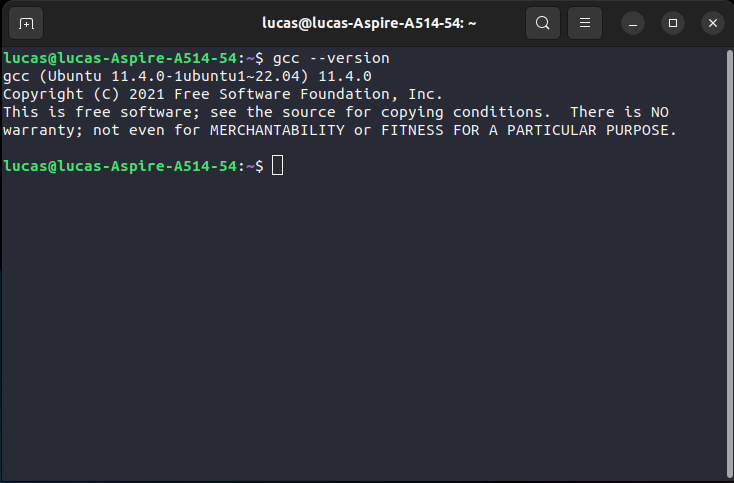
\includegraphics[width=450px]{imagens/versao_gcc.png}
  \end{center}
  \caption{Versão do GCC Sendo exibida no terminal}
  \label{fig:versao_gcc}
\end{figure}

Se o GCC não estiver instalado ou você desejar atualizá-lo para a versão mais recente, siga as etapas apropriadas para a sua distribuição Linux.

\paragraph{Ubuntu e Debian}
No Ubuntu e em sistemas baseados no Debian, você pode usar o \texttt{apt} para instalar o GCC. Abra um terminal e execute os seguintes comandos:
\begin{minted}{bash}
    $ sudo apt update
    $ sudo apt install build-essential
\end{minted}
O pacote \texttt{build-essential} inclui o GCC e outras ferramentas necessárias para compilar programas C.

\paragraph{CentOS e Fedora}
No CentOS e Fedora, você pode usar o \texttt{yum} ou \texttt{dnf} para instalar o GCC. Abra um terminal e execute os seguintes comandos:
\begin{minted}{bash}
    $ sudo yum groupinstall "Development Tools"
\end{minted}

\paragraph{Arch Linux}
No Arch Linux, você pode usar o \texttt{pacman} para instalar o GCC. Abra um terminal e execute o seguinte comando:

\begin{minted}{bash}
    $ sudo pacman -S gcc
\end{minted}

\subsubsection{Windows}
Agora, se você está usando o Windows, uma maneira conveniente de obter um compilador de C é através do Cygwin, que é uma coleção de ferramentas GNU e bibliotecas que fornecem funcionalidades semelhantes às encontradas em sistemas Linux.

Para instalar o Cygwin e o GCC (GNU Compiler Collection) no Windows, siga estas etapas:

\begin{enumerate}
\item Acesse o site oficial do Cygwin em \textbf{https://www.cygwin.com/}

\item Na página inicial do Cygwin, você encontrará um botão para baixar o instalador (normalmente chamado "setup-x86\_64.exe" para sistemas de 64 bits ou "setup-x86.exe" para sistemas de 32 bits). Baixe o instalador apropriado para o seu sistema.

\item Execute o instalador do Cygwin. O instalador irá guiá-lo pelo processo de instalação. Certifique-se de selecionar as opções relevantes, incluindo a seleção do local de instalação e os pacotes que deseja instalar. 

\item Quando chegar à tela de seleção de pacotes, pesquise "gcc" no campo de pesquisa e expanda a categoria "Devel" para encontrar o pacote "gcc-core". Marque a caixa de seleção ao lado dele.

\item Continue com o processo de instalação e o Cygwin instalará o GCC juntamente com outras ferramentas e bibliotecas necessárias.
\end{enumerate}

Para verificar se a instalação foi um sucesso, utilize no Prompt de Comando o seguinte comando que deverá retornar a versão do GCC:

\begin{minted}{bash}
    > gcc --version
\end{minted}

\subsection{Hello World}
Para começar, incluímos a biblioteca padrão de entrada e saída em C, chamada \texttt{<stdio.h>}, usando a diretiva de inclusão \texttt{\#include}.

Isso nos permite escrever o código dentro da função principal do arquivo. Na linguagem C, o código pode ser organizado em funções.

Uma função é um conjunto de comandos que executa uma tarefa específica em um módulo de código independente. A função é referenciada pelo programa principal através do nome atribuído a ela. O uso de funções é comum na programação estruturada, pois ajuda a modularizar o programa.

\begin{lstlisting}[language=C]
#include <stdio.h>

int main(){
    printf("Ola mundo.");
    return 0;
}
\end{lstlisting}

A função principal, denominada \texttt{main}, é uma função que retorna um valor inteiro e não aceita argumentos. O código do nosso programa é escrito dentro dessa função.

Dentro da função principal, usamos a função \texttt{printf}, que recebe uma string de formato como entrada, seguida por uma lista de valores, e produz uma string de saída que corresponde ao especificador de formato e aos valores de entrada fornecidos. Essa função permite exibir valores de qualquer tipo de dado na tela.

\begin{figure}[H]
    \begin{center}
  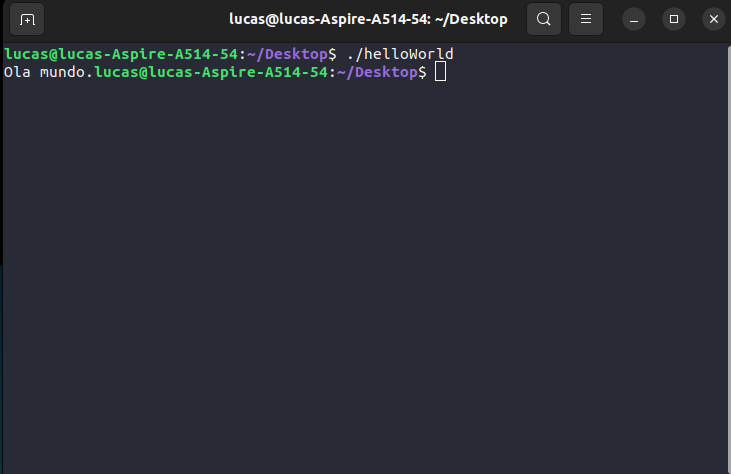
\includegraphics[width=450px]{imagens/hello_world.png}
  \end{center}
  \caption{"Hello World" executado}
  \label{fig:hello_world}
\end{figure}

É importante mencionar que a função principal deve retornar 0 para indicar que o programa foi executado com sucesso. Um retorno de 1 indica erro no código. Portanto, adicionamos a instrução \texttt{return 0;} no final da função principal.
\section{Exercícios}

\subsection{O paradigma imperativo é baseado na ideia de que o computador é uma máquina que executa instruções sequencialmente. Como essa ideia pode ser aplicada para resolver problemas do mundo real?}

A ideia de que o computador é uma máquina que executa instruções sequencialmente pode ser aplicada para resolver problemas do mundo real de várias maneiras. Por exemplo, podemos usar essa ideia para modelar o comportamento de sistemas físicos, como um carro ou um avião. Em um carro, por exemplo, podemos usar instruções sequenciais para representar as ações do motorista, como acelerar, frear e mudar de marcha.

Também podemos usar essa ideia para modelar sistemas lógicos, como um algoritmo ou um programa de computador. Em um algoritmo de ordenação, por exemplo, podemos usar instruções sequenciais para representar as etapas do algoritmo, como comparar dois elementos e trocar sua posição se necessário.

Em geral, podemos usar a ideia de instruções sequenciais para representar qualquer processo que possa ser descrito como uma sequência de passos.

\subsection{O paradigma imperativo é geralmente mais eficiente do que outros paradigmas. Por que isso acontece?}

O paradigma imperativo é mais eficiente do que outros paradigmas porque é baseado no modelo de computação de Von Neumann, que é o modelo mais utilizado em computadores modernos. Esse modelo consiste em uma CPU, uma memória e um conjunto de dispositivos de entrada e saída.

O paradigma imperativo se encaixa bem nesse modelo porque permite aos programadores controlar explicitamente o fluxo de execução do programa, usando instruções como loops e condicionais. Isso permite que os programadores optimizem o código para que seja executado de forma eficiente.

Por exemplo, um programa imperativo que precisa executar um loop 100 vezes pode ser otimizado para que o loop seja executado apenas uma vez, usando uma instrução condicional. Isso pode resultar em uma melhoria significativa no desempenho do programa.

Outros paradigmas, como a programação orientada a objetos, não se encaixam tão bem no modelo de computação de Von Neumann. Isso pode dificultar a otimização do código para que seja executado de forma eficiente.

\subsection{O paradigma imperativo pode ser complexo para problemas grandes e complexos. Quais são algumas estratégias que podem ser usadas para reduzir a complexidade do código imperativo?}

Algumas estratégias que podem ser usadas para reduzir a complexidade do código imperativo incluem:

Modularização: a modularização consiste em dividir o código em módulos menores, cada um com uma função específica. Isso pode ajudar a tornar o código mais fácil de entender e manter.
Abstração: a abstração consiste em ocultar detalhes irrelevantes do código. Isso pode ajudar a tornar o código mais conciso e fácil de entender.
Reutilização de código: a reutilização de código consiste em usar código existente em vez de escrever código novo sempre que necessário. Isso pode ajudar a reduzir a quantidade de código que precisa ser escrito e mantido.
Essas estratégias podem ajudar a tornar o código imperativo mais fácil de entender, manter e estender.

\subsection{O paradigma imperativo pode não ser ideal para problemas grandes e escaláveis. Quais são algumas características dos problemas grandes e escaláveis que tornam o paradigma imperativo menos adequado?}

Algumas características dos problemas grandes e escaláveis que tornam o paradigma imperativo menos adequado incluem:

A necessidade de paralelização: muitos problemas grandes e escaláveis precisam ser executados em paralelo para serem executados de forma eficiente. O paradigma imperativo não fornece suporte nativo para a paralelização, o que pode dificultar a implementação desses problemas.
A complexidade: problemas grandes e escaláveis podem ser muito complexos para serem representados de forma eficiente usando o paradigma imperativo. Isso pode dificultar a implementação desses problemas e pode levar a problemas de desempenho.

\subsection{O paradigma imperativo é o paradigma mais familiar para a maioria dos programadores. Por que isso acontece?}

O paradigma imperativo é o paradigma mais familiar para a maioria dos programadores porque é o paradigma mais antigo e mais amplamente utilizado. O paradigma imperativo foi desenvolvido na década de 1940 e tornou-se o paradigma dominante na programação na década de 1960.

O paradigma imperativo é familiar para os programadores porque é baseado na forma como as pessoas pensam sobre a resolução de problemas. O paradigma imperativo permite que os programadores pensem sobre os problemas como uma sequência de passos, o que é natural para as pessoas.

Também é importante notar que o paradigma imperativo é o paradigma mais ensinado nas escolas e universidades. Isso significa que a maioria dos programadores aprende o paradigma imperativo primeiro, o que torna esse paradigma mais familiar.

Essas são apenas algumas das respostas possíveis para essas perguntas. As respostas específicas podem variar dependendo da interpretação do aluno e do conhecimento que o aluno já possui sobre o paradigma imperativo.


\nocite{linguagemc2023}
\nocite{itsfoss2023}
\nocite{gcc2023}
\nocite{sebesta2018conceitos}
\nocite{codeblocks}

% \section{Submission of papers to TMLR}

% TMLR requires electronic submissions, processed by
% \url{https://openreview.net/}. See TMLR's website for more instructions.

% If your paper is ultimately accepted, use option {\tt accepted} with the {\tt tmlr} 
% package to adjust the format to the camera ready requirements, as follows:
% \begin{center}  
%   {\tt {\textbackslash}usepackage[accepted]\{tmlr\}}. 
% \end{center}
% You also need to specify the month and year
% by defining variables {\tt month} and {\tt year}, which respectively
% should be a 2-digit and 4-digit number. To de-anonymize and remove mentions
% to TMLR (for example for posting to preprint servers), use the preprint option,
% as in {\tt {\textbackslash}usepackage[preprint]\{tmlr\}}. 

% Please read carefully the instructions below, and follow them
% faithfully.

% \subsection{Style}

% Papers to be submitted to TMLR must be prepared according to the
% instructions presented here.

% Authors are required to use the TMLR \LaTeX{} style files obtainable at the
% TMLR website. Please make sure you use the current files and
% not previous versions. Tweaking the style files may be grounds for rejection.

% \subsection{Retrieval of style files}

% The style files for TMLR and other journal information are available online on
% the TMLR website.
% The file \verb+tmlr.pdf+ contains these
% instructions and illustrates the
% various formatting requirements your TMLR paper must satisfy.
% Submissions must be made using \LaTeX{} and the style files
% \verb+tmlr.sty+ and \verb+tmlr.bst+ (to be used with \LaTeX{}2e). The file
% \verb+tmlr.tex+ may be used as a ``shell'' for writing your paper. All you
% have to do is replace the author, title, abstract, and text of the paper with
% your own.

% The formatting instructions contained in these style files are summarized in
% sections \ref{gen_inst}, \ref{headings}, and \ref{others} below.

% \section{General formatting instructions}
% \label{gen_inst}

% The text must be confined within a rectangle 6.5~inches wide and
% 9~inches long. The left margin is 1~inch.
% Use 10~point type with a vertical spacing of 11~points. Computer Modern Bright is the
% preferred typeface throughout. Paragraphs are separated by 1/2~line space,
% with no indentation.

% Paper title is 17~point, in bold and left-aligned.
% All pages should start at 1~inch from the top of the page.

% Authors' names are
% set in boldface. Each name is placed above its corresponding
% address and has its corresponding email contact on the same line, in italic 
% and right aligned. The lead author's name is to be listed first, and
% the co-authors' names are set to follow vertically.

% Please pay special attention to the instructions in section \ref{others}
% regarding figures, tables, acknowledgments, and references.

% \section{Headings: first level}
% \label{headings}

% First level headings are in bold,
% flush left and in point size 12. One line space before the first level
% heading and 1/2~line space after the first level heading.

% \subsection{Headings: second level}

% Second level headings are in bold,
% flush left and in point size 10. One line space before the second level
% heading and 1/2~line space after the second level heading.

% \subsubsection{Headings: third level}

% Third level headings are in bold,
% flush left and in point size 10. One line space before the third level
% heading and 1/2~line space after the third level heading.

% \section{Citations, figures, tables, references}
% \label{others}

% These instructions apply to everyone, regardless of the formatter being used.

% \subsection{Citations within the text}

% Citations within the text should be based on the \texttt{natbib} package
% and include the authors' last names and year (with the ``et~al.'' construct
% for more than two authors). When the authors or the publication are
% included in the sentence, the citation should not be in parenthesis, using \verb|\citet{}| (as
% in ``See \citet{Hinton06} for more information.''). Otherwise, the citation
% should be in parenthesis using \verb|\citep{}| (as in ``Deep learning shows promise to make progress
% towards AI~\citep{Bengio+chapter2007}.'').

% The corresponding references are to be listed in alphabetical order of
% authors, in the \textbf{References} section. As to the format of the
% references themselves, any style is acceptable as long as it is used
% consistently.

% \subsection{Footnotes}

% Indicate footnotes with a number\footnote{Sample of the first footnote} in the
% text. Place the footnotes at the bottom of the page on which they appear.
% Precede the footnote with a horizontal rule of 2~inches.\footnote{Sample of the second footnote}

% \subsection{Figures}

% All artwork must be neat, clean, and legible. Lines should be dark
% enough for purposes of reproduction; art work should not be
% hand-drawn. The figure number and caption always appear after the
% figure. Place one line space before the figure caption, and one line
% space after the figure. The figure caption is lower case (except for
% first word and proper nouns); figures are numbered consecutively.

% Make sure the figure caption does not get separated from the figure.
% Leave sufficient space to avoid splitting the figure and figure caption.

% You may use color figures.
% However, it is best for the
% figure captions and the paper body to make sense if the paper is printed
% either in black/white or in color.
% \begin{figure}[h]
% \begin{center}
% %\framebox[4.0in]{$\;$}
% \fbox{\rule[-.5cm]{0cm}{4cm} \rule[-.5cm]{4cm}{0cm}}
% \end{center}
% \caption{Sample figure caption.}
% \end{figure}

% \subsection{Tables}

% All tables must be centered, neat, clean and legible. Do not use hand-drawn
% tables. The table number and title always appear before the table. See
% Table~\ref{sample-table}. Place one line space before the table title, one line space after the table
% title, and one line space after the table. The table title must be lower case
% (except for first word and proper nouns); tables are numbered consecutively.

% \begin{table}[t]
% \caption{Sample table title}
% \label{sample-table}
% \begin{center}
% \begin{tabular}{ll}
% \multicolumn{1}{c}{\bf PART}  &\multicolumn{1}{c}{\bf DESCRIPTION}
% \\ \hline \\
% Dendrite         &Input terminal \\
% Axon             &Output terminal \\
% Soma             &Cell body (contains cell nucleus) \\
% \end{tabular}
% \end{center}
% \end{table}

% \section{Default Notation}

% In an attempt to encourage standardized notation, we have included the
% notation file from the textbook, \textit{Deep Learning}
% \cite{goodfellow2016deep} available at
% \url{https://github.com/goodfeli/dlbook_notation/}.  Use of this style
% is not required and can be disabled by commenting out
% \texttt{math\_commands.tex}.


% \centerline{\bf Numbers and Arrays}
% \bgroup
% \def\arraystretch{1.5}
% \begin{tabular}{p{1in}p{3.25in}}
% $\displaystyle a$ & A scalar (integer or real)\\
% $\displaystyle \va$ & A vector\\
% $\displaystyle \mA$ & A matrix\\
% $\displaystyle \tA$ & A tensor\\
% $\displaystyle \mI_n$ & Identity matrix with $n$ rows and $n$ columns\\
% $\displaystyle \mI$ & Identity matrix with dimensionality implied by context\\
% $\displaystyle \ve^{(i)}$ & Standard basis vector $[0,\dots,0,1,0,\dots,0]$ with a 1 at position $i$\\
% $\displaystyle \text{diag}(\va)$ & A square, diagonal matrix with diagonal entries given by $\va$\\
% $\displaystyle \ra$ & A scalar random variable\\
% $\displaystyle \rva$ & A vector-valued random variable\\
% $\displaystyle \rmA$ & A matrix-valued random variable\\
% \end{tabular}
% \egroup
% \vspace{0.25cm}

% \centerline{\bf Sets and Graphs}
% \bgroup
% \def\arraystretch{1.5}

% \begin{tabular}{p{1.25in}p{3.25in}}
% $\displaystyle \sA$ & A set\\
% $\displaystyle \R$ & The set of real numbers \\
% $\displaystyle \{0, 1\}$ & The set containing 0 and 1 \\
% $\displaystyle \{0, 1, \dots, n \}$ & The set of all integers between $0$ and $n$\\
% $\displaystyle [a, b]$ & The real interval including $a$ and $b$\\
% $\displaystyle (a, b]$ & The real interval excluding $a$ but including $b$\\
% $\displaystyle \sA \backslash \sB$ & Set subtraction, i.e., the set containing the elements of $\sA$ that are not in $\sB$\\
% $\displaystyle \gG$ & A graph\\
% $\displaystyle \parents_\gG(\ervx_i)$ & The parents of $\ervx_i$ in $\gG$
% \end{tabular}
% \vspace{0.25cm}


% \centerline{\bf Indexing}
% \bgroup
% \def\arraystretch{1.5}

% \begin{tabular}{p{1.25in}p{3.25in}}
% $\displaystyle \eva_i$ & Element $i$ of vector $\va$, with indexing starting at 1 \\
% $\displaystyle \eva_{-i}$ & All elements of vector $\va$ except for element $i$ \\
% $\displaystyle \emA_{i,j}$ & Element $i, j$ of matrix $\mA$ \\
% $\displaystyle \mA_{i, :}$ & Row $i$ of matrix $\mA$ \\
% $\displaystyle \mA_{:, i}$ & Column $i$ of matrix $\mA$ \\
% $\displaystyle \etA_{i, j, k}$ & Element $(i, j, k)$ of a 3-D tensor $\tA$\\
% $\displaystyle \tA_{:, :, i}$ & 2-D slice of a 3-D tensor\\
% $\displaystyle \erva_i$ & Element $i$ of the random vector $\rva$ \\
% \end{tabular}
% \egroup
% \vspace{0.25cm}


% \centerline{\bf Calculus}
% \bgroup
% \def\arraystretch{1.5}
% \begin{tabular}{p{1.25in}p{3.25in}}
% % NOTE: the [2ex] on the next line adds extra height to that row of the table.
% % Without that command, the fraction on the first line is too tall and collides
% % with the fraction on the second line.
% $\displaystyle\frac{d y} {d x}$ & Derivative of $y$ with respect to $x$\\ [2ex]
% $\displaystyle \frac{\partial y} {\partial x} $ & Partial derivative of $y$ with respect to $x$ \\
% $\displaystyle \nabla_\vx y $ & Gradient of $y$ with respect to $\vx$ \\
% $\displaystyle \nabla_\mX y $ & Matrix derivatives of $y$ with respect to $\mX$ \\
% $\displaystyle \nabla_\tX y $ & Tensor containing derivatives of $y$ with respect to $\tX$ \\
% $\displaystyle \frac{\partial f}{\partial \vx} $ & Jacobian matrix $\mJ \in \R^{m\times n}$ of $f: \R^n \rightarrow \R^m$\\
% $\displaystyle \nabla_\vx^2 f(\vx)\text{ or }\mH( f)(\vx)$ & The Hessian matrix of $f$ at input point $\vx$\\
% $\displaystyle \int f(\vx) d\vx $ & Definite integral over the entire domain of $\vx$ \\
% $\displaystyle \int_\sS f(\vx) d\vx$ & Definite integral with respect to $\vx$ over the set $\sS$ \\
% \end{tabular}
% \egroup
% \vspace{0.25cm}

% \centerline{\bf Probability and Information Theory}
% \bgroup
% \def\arraystretch{1.5}
% \begin{tabular}{p{1.25in}p{3.25in}}
% $\displaystyle P(\ra)$ & A probability distribution over a discrete variable\\
% $\displaystyle p(\ra)$ & A probability distribution over a continuous variable, or over
% a variable whose type has not been specified\\
% $\displaystyle \ra \sim P$ & Random variable $\ra$ has distribution $P$\\% so thing on left of \sim should always be a random variable, with name beginning with \r
% $\displaystyle  \E_{\rx\sim P} [ f(x) ]\text{ or } \E f(x)$ & Expectation of $f(x)$ with respect to $P(\rx)$ \\
% $\displaystyle \Var(f(x)) $ &  Variance of $f(x)$ under $P(\rx)$ \\
% $\displaystyle \Cov(f(x),g(x)) $ & Covariance of $f(x)$ and $g(x)$ under $P(\rx)$\\
% $\displaystyle H(\rx) $ & Shannon entropy of the random variable $\rx$\\
% $\displaystyle \KL ( P \Vert Q ) $ & Kullback-Leibler divergence of P and Q \\
% $\displaystyle \mathcal{N} ( \vx ; \vmu , \mSigma)$ & Gaussian distribution %
% over $\vx$ with mean $\vmu$ and covariance $\mSigma$ \\
% \end{tabular}
% \egroup
% \vspace{0.25cm}

% \centerline{\bf Functions}
% \bgroup
% \def\arraystretch{1.5}
% \begin{tabular}{p{1.25in}p{3.25in}}
% $\displaystyle f: \sA \rightarrow \sB$ & The function $f$ with domain $\sA$ and range $\sB$\\
% $\displaystyle f \circ g $ & Composition of the functions $f$ and $g$ \\
%   $\displaystyle f(\vx ; \vtheta) $ & A function of $\vx$ parametrized by $\vtheta$.
%   (Sometimes we write $f(\vx)$ and omit the argument $\vtheta$ to lighten notation) \\
% $\displaystyle \log x$ & Natural logarithm of $x$ \\
% $\displaystyle \sigma(x)$ & Logistic sigmoid, $\displaystyle \frac{1} {1 + \exp(-x)}$ \\
% $\displaystyle \zeta(x)$ & Softplus, $\log(1 + \exp(x))$ \\
% $\displaystyle || \vx ||_p $ & $\normlp$ norm of $\vx$ \\
% $\displaystyle || \vx || $ & $\normltwo$ norm of $\vx$ \\
% $\displaystyle x^+$ & Positive part of $x$, i.e., $\max(0,x)$\\
% $\displaystyle \1_\mathrm{condition}$ & is 1 if the condition is true, 0 otherwise\\
% \end{tabular}
% \egroup
% \vspace{0.25cm}



% \section{Final instructions}
% Do not change any aspects of the formatting parameters in the style files.
% In particular, do not modify the width or length of the rectangle the text
% should fit into, and do not change font sizes (except perhaps in the
% \textbf{References} section; see below). Please note that pages should be
% numbered.

% \section{Preparing PostScript or PDF files}

% Please prepare PostScript or PDF files with paper size ``US Letter'', and
% not, for example, ``A4''. The -t
% letter option on dvips will produce US Letter files.

% Consider directly generating PDF files using \verb+pdflatex+
% (especially if you are a MiKTeX user).
% PDF figures must be substituted for EPS figures, however.

% Otherwise, please generate your PostScript and PDF files with the following commands:
% \begin{verbatim}
% dvips mypaper.dvi -t letter -Ppdf -G0 -o mypaper.ps
% ps2pdf mypaper.ps mypaper.pdf
% \end{verbatim}

% \subsection{Margins in LaTeX}

% Most of the margin problems come from figures positioned by hand using
% \verb+\special+ or other commands. We suggest using the command
% \verb+\includegraphics+
% from the graphicx package. Always specify the figure width as a multiple of
% the line width as in the example below using .eps graphics
% \begin{verbatim}
%    \usepackage[dvips]{graphicx} ...
%    \includegraphics[width=0.8\linewidth]{myfile.eps}
% \end{verbatim}
% or % Apr 2009 addition
% \begin{verbatim}
%    \usepackage[pdftex]{graphicx} ...
%    \includegraphics[width=0.8\linewidth]{myfile.pdf}
% \end{verbatim}
% for .pdf graphics.
% See section~4.4 in the graphics bundle documentation (\url{http://www.ctan.org/tex-archive/macros/latex/required/graphics/grfguide.ps})

% A number of width problems arise when LaTeX cannot properly hyphenate a
% line. Please give LaTeX hyphenation hints using the \verb+\-+ command.

% \subsubsection*{Broader Impact Statement}
% In this optional section, TMLR encourages authors to discuss possible repercussions of their work,
% notably any potential negative impact that a user of this research should be aware of. 
% Authors should consult the TMLR Ethics Guidelines available on the TMLR website
% for guidance on how to approach this subject.

% \subsubsection*{Author Contributions}
% If you'd like to, you may include a section for author contributions as is done
% in many journals. This is optional and at the discretion of the authors. Only add
% this information once your submission is accepted and deanonymized. 

% \subsubsection*{Acknowledgments}
% Use unnumbered third level headings for the acknowledgments. All
% acknowledgments, including those to funding agencies, go at the end of the paper.
% Only add this information once your submission is accepted and deanonymized. 

\bibliography{main}
\bibliographystyle{tmlr}

\end{document}
